%%%%%%%%%%%%%%%%%%%%%%%%%%%%%%%%%%%%%%%%%%%%%%%%%%%%%%%%%%%%%%%%%%%%%%%%%%%%%%
% CS240: Programming in C
% Copyright 2016 Pejman Ghorbanzade <mail@ghorbanzade.com>
% Creative Commons Attribution-ShareAlike 4.0 International License
% https://github.com/ghorbanzade/UMB-CS240-2016S/blob/master/LICENSE
%%%%%%%%%%%%%%%%%%%%%%%%%%%%%%%%%%%%%%%%%%%%%%%%%%%%%%%%%%%%%%%%%%%%%%%%%%%%%%

\def \topDirectory {../..}
\def \texDirectory {\topDirectory/src/main/tex}

\documentclass[compress]{beamer}
%\mode<presentation>
%\usetheme{default}

\usepackage{\texDirectory/template/style/directives}
%%%%%%%%%%%%%%%%%%%%%%%%%%%%%%%%%%%%%%%%%%%%%%%%%%%%%%%%%%%%%%%%%%%%%%%%%%%%%%
% CS114: Introduction to Programming in Java
% Copyright 2015 Pejman Ghorbanzade <mail@ghorbanzade.com>
% Creative Commons Attribution-ShareAlike 4.0 International License
% https://github.com/ghorbanzade/UMB-CS114-2015F/blob/master/LICENSE
%%%%%%%%%%%%%%%%%%%%%%%%%%%%%%%%%%%%%%%%%%%%%%%%%%%%%%%%%%%%%%%%%%%%%%%%%%%%%%

\course{id}{CS240}
\course{name}{Programming in C}
\course{venue}{Mon/Wed, 5:30 PM - 6:45 PM}
\course{semester}{Spring 2016}
\course{department}{Department of Computer Science}
\course{university}{University of Massachusetts Boston}

\instructor{name}{Pejman Ghorbanzade}
\instructor{title}{}
\instructor{position}{Student Instructor}
\instructor{email}{pejman@cs.umb.edu}
\instructor{phone}{617-287-6419}
\instructor{office}{S-3-124B}
\instructor{office-hours}{Mon/Wed 16:00-17:30}
\instructor{address}{University of Massachusetts Boston, 100 Morrissey Blvd., Boston, MA}

\usepackage{\texDirectory/template/style/beamerthemePejman}
\doc{number}{2}
%\setbeamertemplate{footline}[text line]{}

\begin{document}

\prepareCover

\section{Introduction to Unix}

\begin{slide}
	\begin{block}{Multics: Where it all began}

	Multics (Multiplexed Information and Computing Service) was the first time-sharing operating system developed by MIT, Bell Labs and General Electrics.

	\begin{itemize}
	\item[] Introduced in 1964
	\item[] Designed for GE-645 mainframes
	\item[] Modular Hardware Structure
	\item[] Complicated File System
	\item[] Complicated Access Control Policies
	\end{itemize}

	\end{block}
\end{slide}

\begin{slide}
	\begin{columns}

	\column{0.6\textwidth}
	\begin{block}{PDP-7: Where it all began}

	\begin{itemize}
	\item[] Introduced in 1965
	\item[] Only \$72,000
	\item[] 9 KB memory
	\end{itemize}

	Turning point in Computer Science for its role in development of First version of UNIX system and B programming language in 1969 by Ken Thompson.

	\end{block}

	\column{0.4\textwidth}
	\begin{figure}
	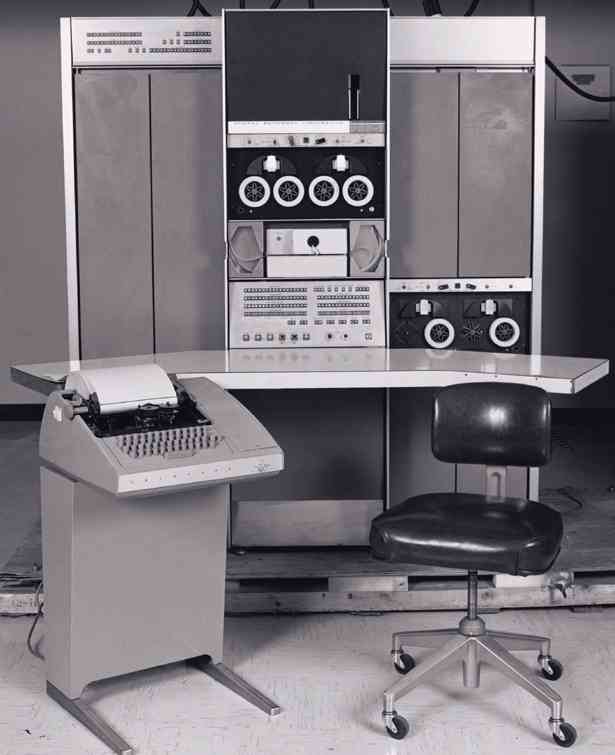
\includegraphics[width=0.8\textwidth]{\texDirectory/img/pdp7.jpg}
	\caption{PDP-7}
	\end{figure}

	\end{columns}
\end{slide}

\begin{slide}
	\begin{block}{Motivations}

	Unics (Uniplex Information and Computing Service) was a rethinked version of Multics operating system, developed by almost the same engineering team to acheive the following:

	\begin{itemize}
	\item[] Portability
	\item[] Multi-tasking
	\item[] Time-sharing
	\end{itemize}

	\end{block}
\end{slide}

\begin{slide}
	\begin{block}{Features}

	\begin{itemize}
	\item[] \alert{Simplicity}
	\item[] Hierarchical File System
	\item[] Multi-user Support
	\item[] Powerful Multi-tasking
	\item[] Powerful Software Architecture
	\end{itemize}

	\end{block}
\end{slide}

\begin{slide}
	\begin{block}{Variants}

	\begin{columns}
	\column{0.5\textwidth}
		\begin{itemize}
		\item[] BSD
		\item[] Solaris
		\item[] Xenis
		\end{itemize}
	\column{0.5\textwidth}
		\begin{itemize}
		\item[] HP-UX
		\item[] Mac OS X
		\item[] Linux
		\end{itemize}
	\end{columns}

	\end{block}
\end{slide}

\begin{slide}
	\begin{block}{Key Components}

	\begin{itemize}
	\item[] Kernel
	\item[] Shell
	\item[] Applications
	\end{itemize}

	\end{block}
\end{slide}

\begin{slide}
	\begin{block}{File System Element Types}

	\begin{columns}
	\column{0.5\textwidth}
		\begin{itemize}
		\item[] file
		\item[] directory
		\item[] link
		\item[] named pipe
		\end{itemize}
	\column{0.5\textwidth}
		\begin{itemize}
		\item[] block device
		\item[] character device
		\item[] socket
		\item[] unknown
		\end{itemize}
	\end{columns}

	\end{block}
\end{slide}

\begin{slide}
	\begin{block}{What is a file?}

	A file is a sequence of bytes that is terminated by the End of File (EOF) character.

	A file is placed in one and only one directory.

	Size of a file is determined by the number of bytes written in it plus a fixed-size file header.

	\end{block}
\end{slide}

\begin{slide}
	\begin{block}{What is a directory?}

	A directory is a file system element that may contain a set of file system elements.

	A directory is placed either in file system root or in one and only one other directory.

	Size of a directory is size of its header.

	\end{block}
\end{slide}

\begin{slide}
	\begin{block}{What is a link?}

	A link is a file system element that points to another file system element.

	Size of a link is size of its header.

	\end{block}
\end{slide}

\begin{slide}
	\begin{block}{Basic Shell Commands}

	\begin{columns}
	\column{0.5\textwidth}
		\begin{itemize}
		\item[] cat
		\item[] cd
		\item[] cp
		\item[] ln
		\item[] ls
		\item[] mkdir
		\end{itemize}
	\column{0.5\textwidth}
		\begin{itemize}
		\item[] mv
		\item[] pwd
		\item[] rm
		\item[] rmdir
		\item[] touch
		\item[] vi
		\end{itemize}
	\end{columns}

	\end{block}
\end{slide}

\begin{slide}
	\begin{block}{Check the \texttt{man} page!}

	\begin{figure}
	
\includegraphics[width=0.8\textwidth]{\texDirectory/img/man-page.jpg}
	\end{figure}

	\end{block}
\end{slide}

\end{document}
